\chapter{Physical layer}\label{sec:physical_layer}

This chapter contains the specification of the supported physical layers of UAVCAN,
as well as some related hardware design recommendations.

Following the requirements and recommendations of this chapter will ensure the highest level of
inter-vendor compatibility and allow the developers to avoid many common design pitfalls.

The sections that provide transport-specific physical layer specification
directly correspond to those defined in the chapter \ref{sec:transport_layer}.

% Please keep \clearpage in front of every transport-specific specification to enforce clear separation!
\clearpage\section{UAVCAN/CAN}\label{sec:transport_can}

\hyphenation{UAVCAN/CAN}  % Disable hyphenation.

This section specifies a concrete transport based on CAN 2.0B (ISO 11898).
Throughout this section, ``CAN'' implies both Classic CAN 2.0 and CAN FD, unless specifically noted otherwise.
CAN FD should be considered the primary transport protocol.

\begin{UAVCANSimpleTable}{UAVCAN/CAN transport capabilities}{|l X l|}
    \label{table:transport_can_capabilities}
    Parameter & Value & References \\

    Maximum node-ID value &
    127 (7 bits wide). &
    \ref{sec:basic} \\

    Transfer-ID mode &
    Cyclic, modulo 32. &
    \ref{sec:transport_transfer_id} \\

    Number of transfer priority levels &
    8 (no additional levels). &
    \ref{sec:transport_transfer_priority} \\

    Largest single-frame transfer payload &
    Classic CAN -- 7~bytes, CAN FD -- up to 63~bytes. &
    \ref{sec:transport_transfer_payload} \\

    Anonymous transfers &
    Supported with non-deterministic collision resolution policy. &
    \ref{sec:transport_route_specifier} \\
\end{UAVCANSimpleTable}

\subsection{CAN ID field}

UAVCAN/CAN transport frames are CAN 2.0B frames.
The 29-bit CAN ID encodes the session specifier\footnote{Section \ref{sec:transport_session_specifier}.}
of the transfer it belongs to along with its priority.
The CAN data field of every frame contains the transfer payload
(or, in the case of multi-frame transfers, a fraction thereof), the transfer-ID, and other metadata.

UAVCAN/CAN can share the same bus with other high-level CAN bus protocols provided that they
do not make use of CAN 2.0B frames\footnote{For example, CANOpen or CANaerospace.}.
However, future revisions of UAVCAN/CAN may utilize CAN 2.0A as well,
so backward compatibility with other high-level CAN bus protocols is not guaranteed.

UAVCAN/CAN can share the same bus with UAVCAN/CAN v0 -- the earlier experimental revision of the protocol
(not recommended for new designs).
The protocol version can be determined at runtime on a per-frame basis as described
in section~\ref{sec:transport_can_toggle_bit}.

UAVCAN/CAN utilizes two different CAN ID bit layouts for message transfers and service transfers.
The bit layouts are summarized on figure~\ref{fig:transport_can_id_structure}.
Tables \ref{table:transport_can_id_fields_message_transfer} and \ref{table:transport_can_id_fields_service_transfer}
summarize the purpose of each field and their permitted values
for message transfers and service transfers, respectively.

% Please do not remove the hard placement specifier [H], it is needed to keep elements ordered.
\begin{figure}[H]
    \centering
    \resizebox{\textwidth}{!}{
        \footnotesize
        \begin{tabular}{|l|c|c|c|c|c|c|c|c|c|c|c|c|c|c|c|c|c|c|c|c|c|c|c|c|c|c|c|c|c|} \hline
            %
            % Message transfer
            %
            \multirow{2}{*}{\textbf{Message}} &
            \multicolumn{4}{c|}{Service, not message} &
            \multicolumn{3}{c|}{Anonymous} &
            \multicolumn{14}{c|}{\multirow{2}{*}{Subject-ID}} &
            \multicolumn{1}{c|}{\multirow{2}{*}{R}} &
            \multicolumn{7}{c|}{\multirow{2}{*}{Source node-ID}}
            \\\cline{2-4} \cline{7-8}

            &
            \multicolumn{3}{c|}{Priority}
            &
            &
            &
            R &
            \multicolumn{15}{c|}{} &
            &
            \multicolumn{7}{c|}{}
            \\

            \textbf{Values} &
            \multicolumn{3}{c|}{$[0, 7]$} &
            $0$ &
            $\mathbb{B}$ &
            $0$ &
            \multicolumn{1}{c}{} &
            \multicolumn{14}{c|}{$[0, 32767]$} &
            $0$ &
            \multicolumn{7}{c|}{$[0, 127]$}
            \\\hline

            \textbf{CAN ID bit} &
            28 & 27 & 26 & 25 & 24 & 23 & 22 & 21 & 20 & 19 & 18 & 17 & 16 & 15 &
            14 & 13 & 12 & 11 & 10 &  9 &  8 &  7 &  6 &  5 &  4 &  3 &  2 &  1 &  0
            \\\hline

            \textbf{CAN ID byte} &
            \multicolumn{5}{c|}{3} & \multicolumn{8}{c|}{2} & \multicolumn{8}{c|}{1} & \multicolumn{8}{c|}{0}
            \\\hline

            \multicolumn{30}{c}{} \\ \hline % Table separator

            %
            % Service transfer
            %
            \multirow{2}{*}{\textbf{Service}} &
            \multicolumn{4}{c|}{Service, not message} &
            \multicolumn{5}{c|}{Request, not response} &
            \multicolumn{6}{c|}{} &
            \multicolumn{7}{c|}{\multirow{2}{*}{Destination node-ID}} &
            \multicolumn{7}{c|}{\multirow{2}{*}{Source node-ID}}
            \\\cline{2-4} \cline{7-10}

            &
            \multicolumn{3}{c|}{Priority} &
            &
            &
            R &
            \multicolumn{9}{c|}{Service-ID} &
            \multicolumn{7}{c|}{} &
            \multicolumn{7}{c|}{}
            \\

            \textbf{Values} &
            \multicolumn{3}{c|}{$[0, 7]$} &
            $1$ &
            $\mathbb{B}$ &
            $0$ &
            \multicolumn{9}{c|}{$[0, 511]$} &
            \multicolumn{7}{c|}{$[0, 127]$} &
            \multicolumn{7}{c|}{$[0, 127]$}
            \\\hline

            \textbf{CAN ID bit} &
            28 & 27 & 26 & 25 & 24 & 23 & 22 & 21 & 20 & 19 & 18 & 17 & 16 & 15 &
            14 & 13 & 12 & 11 & 10 &  9 &  8 &  7 &  6 &  5 &  4 &  3 &  2 &  1 &  0
            \\\hline

            \textbf{CAN ID byte} &
            \multicolumn{5}{c|}{3} & \multicolumn{8}{c|}{2} & \multicolumn{8}{c|}{1} & \multicolumn{8}{c|}{0}
            \\\hline
        \end{tabular}
    }
    \caption{CAN ID bit layout}\label{fig:transport_can_id_structure}
\end{figure}

\begin{UAVCANSimpleTable}{CAN ID bit fields for message transfers}{|l l l X|}
    \label{table:transport_can_id_fields_message_transfer}
    Field               & Width & Valid values  & Description \\

    Transfer priority   & 3     & $[0, 7]$ (any)    & Section \ref{sec:transport_transfer_priority}. \\

    Service not message & 1     & $0$               & Always zero for message transfers. \\

    Anonymous           & 1     & $\{0, 1\}$ (any)  & Zero for regular message transfers,
                                                      one for anonymous transfers. \\

    Reserved bit 23     & 1     & $0$               & Discard frame if this field has a different value. \\

    Subject-ID          & 15    & $[0, 32767]$ (any) & Subject-ID of the current message transfer. \\

    Reserved bit 7      & 1     & $0$               & Discard frame if this field has a different value. \\

    Source node-ID      & 7     & $[0, 127]$ (any)  & Node-ID of the origin.
                                                      For anonymous transfers, this field contains a pseudo-ID instead,
                                                      as described in section
                                                      \ref{sec:transport_can_source_node_pseudo_id}. \\
\end{UAVCANSimpleTable}

\begin{UAVCANSimpleTable}{CAN ID bit fields for service transfers}{|l l l X|}
    \label{table:transport_can_id_fields_service_transfer}
    Field               & Width & Valid values  & Description \\

    Transfer priority   & 3     & $[0, 7]$ (any)    & Section \ref{sec:transport_transfer_priority}. \\

    Service not message & 1     & $1$               & Always one for service transfers. \\

    Request not response& 1     & $\{0, 1\}$ (any)  & One for service request, zero for service response. \\

    Reserved bit 23     & 1     & $0$               & Discard frame if this field has a different value. \\

    Service-ID          & 9     & $[0, 511]$ (any)  & Service-ID of the encoded service object
                                                      (request or response). \\

    Destination node-ID & 7     & $[0, 127]$ (any)  & Node-ID of the destination:
                                                      server if request, client if response. \\

    Source node-ID      & 7     & $[0, 127]$ (any)  & Node-ID of the origin:
                                                      client if request, server if response. \\
\end{UAVCANSimpleTable}

\subsubsection{Transfer priority}

Valid values for transfer priority range from 0 to 7, inclusively,
where 0 corresponds to the highest priority, and 7 corresponds to the lowest priority
(according to the CAN bus arbitration policy).

In multi-frame transfers, the value of the priority field shall be identical for all frames of the transfer.

\begin{remark}[breakable]
    When multiple transfers of different types with the same priority contest for bus access,
    the following precedence is ensured (from higher priority to lower priority):

    \begin{enumerate}
        \item Message transfers (the primary method of data exchange in UAVCAN networks).
        \item Anonymous (message) transfers.
        \item Service response transfers (preempt requests).
        \item Service request transfers (responses take precedence over requests to make service calls more atomic
              and reduce the number of pending states in the system).
    \end{enumerate}

    Mnemonics for transfer priority levels are provided in section \ref{sec:transport_transfer_priority},
    and their mapping to the UAVCAN/CAN priority field is as follows:

    \begin{UAVCANCompactTable}{|l X|}
        Priority field value    & Mnemonic name \\
        0                       & Exceptional   \\
        1                       & Immediate     \\
        2                       & Fast          \\
        3                       & High          \\
        4                       & Nominal       \\
        5                       & Low           \\
        6                       & Slow          \\
        7                       & Optional      \\
    \end{UAVCANCompactTable}

    Since the value of transfer priority is required to be the same for all frames in a transfer,
    it follows that the value of the CAN ID is guaranteed to be the same for all CAN frames of the transfer.
    Given a constant transfer priority value, all CAN frames under a given session specifier will be equal.
\end{remark}

\subsubsection{Source node-ID field in anonymous transfers}\label{sec:transport_can_source_node_pseudo_id}

The source node-ID field of anonymous transfers shall be initialized with a pseudorandom \emph{pseudo-ID} value.
The source of the pseudorandom data used for the pseudo-ID shall aim to produce different values
for different CAN frame data field values.

A node transmitting an anonymous transfer shall abort its transmission and discard it upon detection of a bus error.
Some method of media access control should be used at the application level for further conflict resolution.

\begin{remark}[breakable]
    CAN bus does not allow different nodes to transmit CAN frames with different data under the same CAN ID value.
    Owing to the fact that the CAN ID includes the node-ID of the transmitting node,
    this restriction does not affect non-anonymous transfers.
    However, anonymous transfers would violate this restriction because their source node-ID is not defined,
    hence the additional measures described in this section.

    A possible way of initializing the source node pseudo-ID value is to compute the arithmetic sum
    of all bytes of the transfer payload, taking the least significant bits of the result as the pseudo-ID
    (usage of stronger hashes is encouraged).
    Implementations that adopt this approach will be using the same pseudo-ID value for identical transfer payloads,
    which is acceptable since this will not trigger an error on the bus.

    Because the set of possible pseudo-ID values is small,
    a collision where multiple nodes emit CAN frames with different data but the same CAN ID is likely to happen
    despite the randomization measures described here.
    Therefore, if anonymous transfers are used,
    implementations shall account for possible errors on the CAN bus triggered by CAN ID collisions.

    Automatic retransmission should be disabled for anonymous transfers (like in TTCAN).
    This measure allows the protocol to prevent temporary disruptions that may occur if the automatic
    retransmission on bus error is not suppressed.

    Additional bus access control logic is needed at the application level because
    the possibility of identifier collisions in anonymous frames undermines the access control logic implemented
    in CAN bus controller hardware.

    The described principles make anonymous transfers highly non-deterministic and inefficient.
    This is considered acceptable because the scope of anonymous transfers is limited to a very narrow set of use
    cases which tolerate their downsides. The UAVCAN specification employs anonymous transfers only for the
    plug-and-play feature defined in section \ref{sec:application_functions}.
    Deterministic applications are advised to avoid reliance on anonymous transfers completely.

    None of the above considerations affect nodes that do not transmit anonymous transfers.
\end{remark}

\subsection{CAN data field}

\subsubsection{Layout}

UAVCAN/CAN utilizes a fixed layout of the CAN data field:
the last byte of the CAN data field contains the metadata, it is referred to as the \emph{tail byte}.
The preceding bytes of the data field contain the transfer payload,
which may be extended with padding bytes and transfer CRC.

A CAN frame whose data field contains less than one byte is not a valid UAVCAN/CAN frame.

The bit layout of the tail byte is shown in table \ref{table:transport_can_tail_byte}.

% Please do not remove the hard placement specifier [H], it is needed to keep tables ordered.
\begin{table}[H]\caption{Tail byte structure}\label{table:transport_can_tail_byte}
    \begin{tabu}{| c l | X[c2] X[c3] |}
        \hline
        \rowfont{\bfseries}
        Bit & Field & Single-frame transfers & Multi-frame transfers \\
        \hline
        7   & \textbf{Start of transfer}& Always 1  & First frame: 1, otherwise 0. \\\hline
        6   & \textbf{End of transfer}  & Always 1  & Last frame: 1, otherwise 0. \\\hline
        5   & \textbf{Toggle bit}       & Always 1  & First frame: 1, then alternates;
                                                      section \ref{sec:transport_can_toggle_bit}. \\\hline
        4   &                           & \multicolumn{2}{c|}{} \\
        3   &                           & \multicolumn{2}{c|}{Modulo 32 (range [0, 31])} \\
        2   & \textbf{Transfer-ID}      & \multicolumn{2}{c|}{section \ref{sec:transport_transfer_id}} \\
        1   &                           & \multicolumn{2}{c|}{} \\
        0   &                           & \multicolumn{2}{c|}{\footnotesize{(least significant bit)}} \\
        \hline
    \end{tabu}
\end{table}

\subsubsection{Toggle bit}\label{sec:transport_can_toggle_bit}

Transport frames that form a multi-frame transfer are equipped with a \emph{toggle bit}
which alternates its state every frame within the transfer for frame deduplication purposes\footnote{%
    A frame that appears valid to the receiving node may under certain conditions appear invalid to the transmitter,
    triggering the latter to retransmit the frame, in which case it will be duplicated on the side of the receiver.
}.

\begin{remark}[breakable]
    The toggle bit can be used to facilitate operation of heterogeneous deployments where the experimental
    UAVCAN/CAN v0 shares the same CAN bus with the current version of the standard.

    Whenever a new transfer is initiated, the original state of the toggle bit reflects the protocol version.
    Implementations that need to support simultaneous operation of two versions of the protocol can record
    the state of the toggle bit when the ``start of transfer'' bit is set, and keep this information
    indexed by the value of the CAN ID field (all frames of a transfer are guaranteed to share the same CAN ID).
    The resulting mapping from CAN ID to the protocol version can be used to route incoming frames to the
    implementation of the appropriate version of the protocol.

    \begin{UAVCANSimpleTable}{Protocol version detection based on the toggle bit}{|l l X|}
        Start of transfer   & Toggle bit    & Protocol version \\
        1                   & 0             & UAVCAN v0 (experimental version). \\
        1                   & 1             & UAVCAN v1 (this version). \\
        0                   & x             & Keep the state of the toggle bit from the first frame of the transfer
                                              to detect protocol version in multi-frame transfers. \\
    \end{UAVCANSimpleTable}
\end{remark}

\subsubsection{Transfer payload decomposition}

The transport-layer MTU of Classic CAN-based implementations shall be 8 bytes (the maximum).
The transport-layer MTU of CAN FD-based implementations should be 64 bytes (the maximum).

CAN FD does not guarantee byte-level granularity of the CAN data field length.
If the desired length of the CAN data field cannot be represented due to the granularity constraints,
zero padding bytes are used.

In single-frame transfers, padding bytes are inserted between the end of the payload and the tail byte.

In multi-frame transfers, the transfer payload is appended with trailing zero padding bytes
followed by the transfer CRC (section \ref{sec:transport_can_transfer_crc}).
All transport frames of a multi-frame transfer except the last one shall fully utilize the available
data field capacity; hence, padding is unnecessary there.
The number of padding bytes is computed so that the length granularity constraints
for the last frame of the transfer are satisfied.

\begin{remark}
    Usage of padding bytes implies that when a serialized message is being deserialized by a receiving node,
    the byte sequence used for deserialization may be longer than the actual byte sequence generated by the
    emitting node during serialization.
    This behavior is compatible with the DSDL specification.

    The weak MTU requirement for CAN FD is designed to avoid compatibility issues.
\end{remark}

\subsubsection{Transfer CRC}\label{sec:transport_can_transfer_crc}

Payload of multi-frame transfers is extended with a transfer CRC for validating the correctness of their reassembly.
Transfer CRC is not used with single-frame transfers.

The transfer CRC is computed over the entire payload of the multi-frame transfer
plus the trailing padding bytes, if any.
The resulting CRC value is appended to the transfer payload after the padding bytes (if any)
in the \emph{big-endian byte order} (most significant byte first)\footnote{%
    This is the native byte order for this CRC function.
}.

The CRC function is the standard CRC-16-CCITT:
initial value $\mathrm{FFFF}_{16}$, polynomial $\mathrm{1021}_{16}$,
not reversed, no output XOR, big endian.
The value for an input sequence $\left(49, 50, \ldots, 56, 57\right)$ is $\mathrm{29B1}_{16}$.
The following code snippet provides a basic implementation of the transfer CRC algorithm in C++
(LUT-based alternatives exist).

\begin{samepage}
\begin{minted}{cpp}
#include <cstdint>
#include <cstddef>

/// UAVCAN/CAN transfer CRC function implementation. License: CC0, no copyright reserved.
class CANTransferCRC
{
    std::uint16_t value_ = 0xFFFFU;

public:
    void add(const std::uint8_t byte)
    {
        value_ ^= static_cast<std::uint16_t>(byte) << 8U;
        for (std::uint8_t bit = 8; bit > 0; --bit)
        {
            if ((value_ & 0x8000U) != 0)
            {
                value_ = (value_ << 1U) ^ 0x1021U;
            }
            else
            {
                value_ = value_ << 1U;
            }
        }
    }

    void add(const std::uint8_t* bytes, std::size_t length)
    {
        while (length-- > 0)
        {
            add(*bytes++);
        }
    }

    [[nodiscard]] std::uint16_t get() const { return value_; }
};
\end{minted}
\end{samepage}

\subsection{Examples}

\begin{remark}[breakable]
    Heartbeat from node-ID 42, nominal priority level,
    uptime starting from 0 and then incrementing by one every transfer,
    vendor-specific status code 3471:

    \begin{UAVCANCompactTable}{|l l|}
        CAN ID (hex)      & CAN data (hex)          \\
        \texttt{107D552A} & \texttt{00 00 00 00 04 78 68 E0} \\
        \texttt{107D552A} & \texttt{01 00 00 00 04 78 68 E1} \\
        \texttt{107D552A} & \texttt{02 00 00 00 04 78 68 E2} \\
        \texttt{107D552A} & \texttt{03 00 00 00 04 78 68 E3} \\
    \end{UAVCANCompactTable}

    \verb|uavcan.primitive.String.1.0| under subject-ID 4919 ($1337_{16}$) published by an anonymous node,
    the string is ``\verb|Hello world!|'' (ASCII); one byte of zero padding can be seen between
    the payload and the tail byte:

    \begin{UAVCANCompactTable}{|l l|}
        CAN ID (hex)      & CAN data (hex)                                           \\
        \texttt{11133775} & \texttt{00 18 48 65 6C 6C 6F 20 77 6F 72 6C 64 21 00 E0} \\
        \texttt{11133775} & \texttt{00 18 48 65 6C 6C 6F 20 77 6F 72 6C 64 21 00 E1} \\
        \texttt{11133775} & \texttt{00 18 48 65 6C 6C 6F 20 77 6F 72 6C 64 21 00 E2} \\
        \texttt{11133775} & \texttt{00 18 48 65 6C 6C 6F 20 77 6F 72 6C 64 21 00 E3} \\
    \end{UAVCANCompactTable}

    Node info request from node 123 to node 42 via Classic CAN, then response;
    notice how the transfer CRC is scattered across two frames:

    \begin{UAVCANCompactTable}{|l l l X|}
        CAN ID (hex)      & CAN data (hex)                                  & ASCII             & Comment \\

        \texttt{136B957B} & \texttt{E1}                                     & \texttt{.}        &
        The request contains no payload. \\

        \texttt{126BBDAA} & \texttt{01 00 00 00 01 00 00 A1}                & \texttt{........} &
        Start of response, toggle bit is set. \\

        \texttt{126BBDAA} & \texttt{00 00 00 00 00 00 00 01}                & \texttt{........} &
        Toggle bit is cleared. \\

        \texttt{126BBDAA} & \texttt{00 00 00 00 00 00 00 21}                & \texttt{.......!} &
        Toggle bit is set. \\

        \texttt{126BBDAA} & \texttt{00 00 00 00 00 00 00 01}                & \texttt{........} &
        Etc. \\

        \texttt{126BBDAA} & \texttt{00 00 \underline{24} 6F 72 67 2E 21}    & \texttt{..\underline{\$}org.!} &
        Array (string) length prefix. \\

        \texttt{126BBDAA} & \texttt{75 61 76 63 61 6E 2E 01}                & \texttt{uavcan..} &
        \\

        \texttt{126BBDAA} & \texttt{70 79 75 61 76 63 61 21}                & \texttt{pyuavca!} &
        \\

        \texttt{126BBDAA} & \texttt{6E 2E 64 65 6D 6F 2E 01}                & \texttt{n.demo..} &
        \\

        \texttt{126BBDAA} & \texttt{62 61 73 69 63 5F 75 21}                & \texttt{basic\_u!} &
        \\

        \texttt{126BBDAA} & \texttt{73 61 67 65 00 00 \underline{9A} 01}    & \texttt{sage..\underline{.}.} &
        Transfer CRC, MSB. \\

        \texttt{126BBDAA} & \texttt{\underline{E7} 61}                      & \texttt{\underline{.}a}       &
        Transfer CRC, LSB. \\
    \end{UAVCANCompactTable}

    \verb|uavcan.primitive.array.Natural8.1.0| under subject-ID 4919 ($1337_{16}$) published by node 59,
    the array contains an arithmetic sequence $\left(0, 1, 2, \ldots{}, 89, 90, 91\right)$;
    the transport MTU is 64 bytes:

    \begin{UAVCANCompactTable}{|l X[2] X|}
        CAN ID (hex)      & CAN data (hex) & Comment \\
        \texttt{1013373B} &
        \texttt{%
            00 B8 00 01 02 03 04 05 06 07 08 09 0A 0B 0C 0D 0E 0F 10 11 12 13 14 15 16 17 18 19 1A 1B 1C 1D 1E 1F 20
            21 22 23 24 25 26 27 28 29 2A 2B 2C 2D 2E 2F 30 31 32 33 34 35 36 37 38 39 3A 3B 3C A0
        } &
        First frame: 1.~payload (array length prefix is 92); 2.~tail byte. \\

        \texttt{1013373B} &
        \texttt{%
            3D 3E 3F 40 41 42 43 44 45 46 47 48 49 4A 4B 4C 4D 4E 4F 50 51 52 53 54 55 56 57 58 59 5A 5B
            \underline{00} \underline{00} \underline{00} \underline{00} \underline{00} \underline{00} \underline{00}
            \underline{00} \underline{00} \underline{00} \underline{00} \underline{00} \underline{00} \underline{00}
            \textbf{C0} \textbf{48} 40
        } &
        Last frame: 1.~payload; 2.~padding (underlined); 3.~transfer CRC (bold); 4.~tail byte. \\
    \end{UAVCANCompactTable}
\end{remark}

\subsection{Software design considerations}

\subsubsection{Ordered transmission}

The CAN controller driver software shall guarantee that CAN frames with identical CAN ID values
will be transmitted in their order of appearance in the transmission queue\footnote{%
    This is because multi-frame transfers use identical CAN ID for all frames of the transfer,
    and UAVCAN requires that all frames of a multi-frame transfer shall be transmitted in the correct order.
}.

\subsubsection{Transmission timestamping}

\begin{remark}[breakable]
    Certain application-level functions of UAVCAN may require the driver to timestamp outgoing transport frames,
    e.g., the time synchronization function.
    A sensible approach to transmission timestamping is built around the concept of \emph{loop-back frames},
    which is described here.

    If the application needs to timestamp an outgoing frame, it sets a special flag -- the \emph{loop-back flag} --
    on the frame before sending it to the driver.
    The driver would then automatically re-enqueue this frame back into the reception queue once it is transmitted
    (keeping the loop-back flag set so that the application is able to distinguish the loop-back
    frame from regular received traffic).
    The timestamp of the loop-backed frame would be of the moment when it was delivered to the bus.

    The advantage of the loop-back based approach is that it relies on the same interface between
    the application and the driver that is used for regular communications.
    No complex and dangerous callbacks or write-backs from interrupt handlers are involved.
\end{remark}

\subsubsection{Inner priority inversion}

Implementations should take necessary precautions against the problem of inner priority inversion.

\begin{remark}[breakable]
    Suppose the application needs to emit a frame with the CAN ID $X$.
    The frame is submitted to the CAN controller's registers and the transmission is started.
    Suppose that afterwards it turned out that there is a new frame with the CAN ID $(X-1)$ that needs to be sent,
    too, but the previous frame $X$ is in the way, and it is blocking the transmission of the new frame.
    This may turn into a problem if the lower-priority frame is losing arbitration on the bus due
    to the traffic on the bus having higher priority than the current frame,
    but lower priority than the next frame that is waiting in the queue.

    A naive solution to this is to continuously check whether the priority of the frame that is currently being
    transmitted by the CAN controller is lower than the priority of the next frame in the queue, and if it is,
    abort transmission of the current frame, move it back to the transmission queue,
    and begin transmission of the new one instead.
    This approach, however, has a hidden race condition:
    the old frame may be aborted at the moment when it has already been received by remote nodes,
    which means that the next time it is re-transmitted, the remote nodes will see it duplicated.
    Additionally, this approach increases the complexity of the driver and can possibly affect
    its throughput and latency.

    Most CAN controllers offer a robust solution to the problem:
    they have multiple transmission mailboxes (usually at least 3),
    and the controller always chooses for transmission the mailbox which contains the highest priority frame.
    This provides the application with a possibility to avoid the inner priority inversion problem:
    whenever a new transmission is initiated, the application should check whether the priority of the next frame
    is higher than any of the other frames that are already awaiting transmission.
    If there is at least one higher-priority frame pending,
    the application doesn't move the new one to the controller's transmission mailboxes,
    it remains in the queue.
    Otherwise, if the new frame has a higher priority level than all of the pending frames,
    it is pushed to the controller's transmission mailboxes and removed from the queue.
    In the latter case, if a lower-priority frame loses arbitration,
    the controller would postpone its transmission and try transmitting the higher-priority one instead.
    That resolves the problem.

    There is an interesting extreme case, however.
    Imagine a controller equipped with $N$ transmission mailboxes.
    Suppose the application needs to emit $N$ frames in the increasing order of priority,
    which leads to all of the transmission mailboxes of the controller being occupied.
    Now, if all of the conditions below are satisfied, the system ends up with a priority inversion condition
    nevertheless, despite the measures described above:

    \begin{itemize}
        \item The highest-priority pending CAN frame cannot be transmitted due to the bus being saturated
        with a higher-priority traffic.
        \item The application needs to emit a new frame which has a higher priority than that which saturates the bus.
    \end{itemize}

    If both hold, a priority inversion is afoot because there is no free transmission mailbox to
    inject the new higher-priority frame into.
    The scenario is extremely unlikely, however;
    it is also possible to construct the application in a way that would preclude the problem,
    e.g., by limiting the number of simultaneously used distinct CAN ID values.

    The following pseudocode demonstrates the principles explained above:

    \begin{samepage}
    \begin{minted}{cpp}
    // Returns the index of the TX mailbox that can be used for the transmission of the newFrame
    // If none are available, returns -1.
    getFreeMailboxIndex(newFrame)
    {
        chosen_mailbox = -1     // By default, assume that no mailboxes are available

        for i = 0...NumberOfTxMailboxes
        {
            if isTxMailboxFree(i)
            {
                chosen_mailbox = i
                // Note: cannot break here, shall check all other mailboxes as well.
            }
            else
            {
                if not isFramePriorityHigher(newFrame, getFrameFromTxMailbox(i))
                {
                    chosen_mailbox = -1
                    break   // Denied - shall wait until this mailbox has finished transmitting
                }
            }
        }

        return chosen_mailbox
    }
    \end{minted}
    \end{samepage}
\end{remark}

\subsubsection{Automatic hardware acceptance filter configuration}

\begin{remark}[breakable]
    Most CAN controllers are equipped with hardware acceptance filters.
    Hardware acceptance filters reduce the application workload by ignoring irrelevant CAN frames on the bus
    by comparing their ID values against the set of relevant ID values configured by the application.

    There exist two common approaches to CAN hardware filtering:
    list-based and mask-based.
    In the case of the list-based approach, every CAN frame detected on the bus is compared
    against the set of reference CAN ID values provided by the application;
    only those frames that are found in the reference set are accepted.
    Due to the complex structure of the CAN ID field used by UAVCAN,
    usage of the list-based filtering method with this protocol is impractical.

    Most CAN controller vendors implement mask-based filters,
    where the behavior of each filter is defined by two parameters: the mask $M$ and the reference ID $R$.
    Then, such filter accepts only those CAN frames for which the following bitwise logical condition holds
    true\footnote{Notation: $\land$ -- bitwise logical AND, $\oplus$ -- bitwise logical XOR,
    $\neg$ -- bitwise logical NOT.}:
    $$((X \land M) \oplus R) \leftrightarrow 0$$
    where $X$ is the CAN ID value of the evaluated frame.

    Complex UAVCAN applications are often required to operate with more distinct transfers than there are
    acceptance filters available in the hardware.
    That creates the challenge of finding the optimal configuration of the available filters that meets the
    following criteria:
    \begin{itemize}
        \item All CAN frames needed by the application are accepted.
        \item The number of irrelevant frames (i.e., not used by the application) accepted from the bus is minimized.
    \end{itemize}

    The optimal configuration is a function of the number of available hardware filters,
    the set of distinct transfers needed by the application,
    and the expected frequency of occurrence of all possible distinct transfers on the bus.
    The latter is important because if there are to be irrelevant transfers,
    it makes sense to optimize the configuration so that the acceptance of less common irrelevant transfers
    is preferred over the more common irrelevant transfers, as that reduces the processing load on the application.

    The optimal configuration depends on the properties of the network the node is connected to.
    In the absence of the information about the network,
    or if the properties of the network are expected to change frequently,
    it is possible to resort to a quasi-optimal configuration which assumes that
    the occurrence of all possible irrelevant transfers is equally probable.
    As such, the quasi-optimal configuration is a function of only the number of available hardware filters
    and the set of distinct transfers needed by the application.

    The quasi-optimal configuration can be easily found automatically.
    Certain implementations of the UAVCAN protocol stack include this functionality,
    allowing the application to easily adjust the configuration of the hardware acceptance filters
    using a very simple API.

    A quasi-optimal hardware acceptance filter configuration algorithm is described below.
    The approach was first proposed by P. Kirienko and I. Sheremet in 2015.

    First, the bitwise \emph{filter merge} operation is defined on filter configurations $A$ and $B$.
    The set of CAN frames accepted by the merged filter configuration is a superset of
    those accepted by $A$ and $B$.
    The definition is as follows:
    \begin{equation*}
    \begin{split}
        m_M(R_A, R_B, M_A, M_B) & = M_A \land M_B \land \neg (R_A \oplus R_B) \\
        m_R(R_A, R_B, M_A, M_B) & = R_A \land m_M(R_A, R_B, M_A, M_B)
    \end{split}
    \end{equation*}

    The \emph{filter rank} is a function of the mask of the filter.
    The rank of a filter is a unitless quantity that defines in relative terms how selective the filter
    configuration is.
    The rank of a filter is proportional to the likelihood that the filter will reject a random CAN ID.
    In the context of hardware filtering, this quantity is conveniently representable via the number of bits set in
    the filter mask parameter (also known as \emph{population count}):
    \begin{equation*}
    r(M) =
    \begin{cases}
        0                                   &\mid M < 1 \\
        r(\lfloor\frac{M}{2}\rfloor)        &\mid M \bmod 2 = 0 \\
        r(\lfloor\frac{M}{2}\rfloor) + 1    &\mid M \bmod 2 \neq 0 \\
    \end{cases}
    \end{equation*}

    Having the low-level operations defined, we can proceed to define the whole algorithm.
    First, construct the initial set of CAN acceptance filter configurations
    according to the requirements of the application.
    Then, as long as the number of configurations in the set exceeds the number of available
    hardware acceptance filters, repeat the following:
    \begin{enumerate}
        \item Find the pair $A$, $B$ of configurations in the set for which $r(m_M(R_A, R_B, M_A, M_B))$ is maximized.
        \item Remove $A$ and $B$ from the set of configurations.
        \item Add a new configuration $X$ to the set of configurations, where
        $M_X = m_M(R_A, R_B, M_A, M_B)$, and $R_X = m_R(R_A, R_B, M_A, M_B)$.
    \end{enumerate}

    The algorithm reduces the number of filter configurations by one at each iteration,
    until the number of available hardware filters is sufficient to accommodate the whole set of configurations.
\end{remark}


\clearpage
\section{Hardware design recommendations}

This section contains certain generic hardware design recommendations that are agnostic of a particular
physical layer implementation.

\subsection{Non-uniform transport redundancy}\label{sec:phy_non_uniform_transport_redundancy}

Mission critical devices and non-mission critical devices often need to co-exist within the same UAVCAN network.
Non-mission critical devices are likely to be equipped with a non-redundant transport interface,
which can create a situation where multiple devices with different numbers of redundant interfaces
need to be connected to the same network.
In that case, the following rules should be followed:

\begin{itemize}
    \item Each available bus is assigned a level of importance (primary, secondary, etc.).
    \item All nodes should be connected to the primary bus.
    \item Only nodes with redundant interfaces should be also connected to the non-primary bus/buses.
\end{itemize}

The figure \ref{fig:phy_non_uniform_transport_redundancy} shows a doubly redundant bus transport as an example.

\begin{figure}[H]
    \centering
	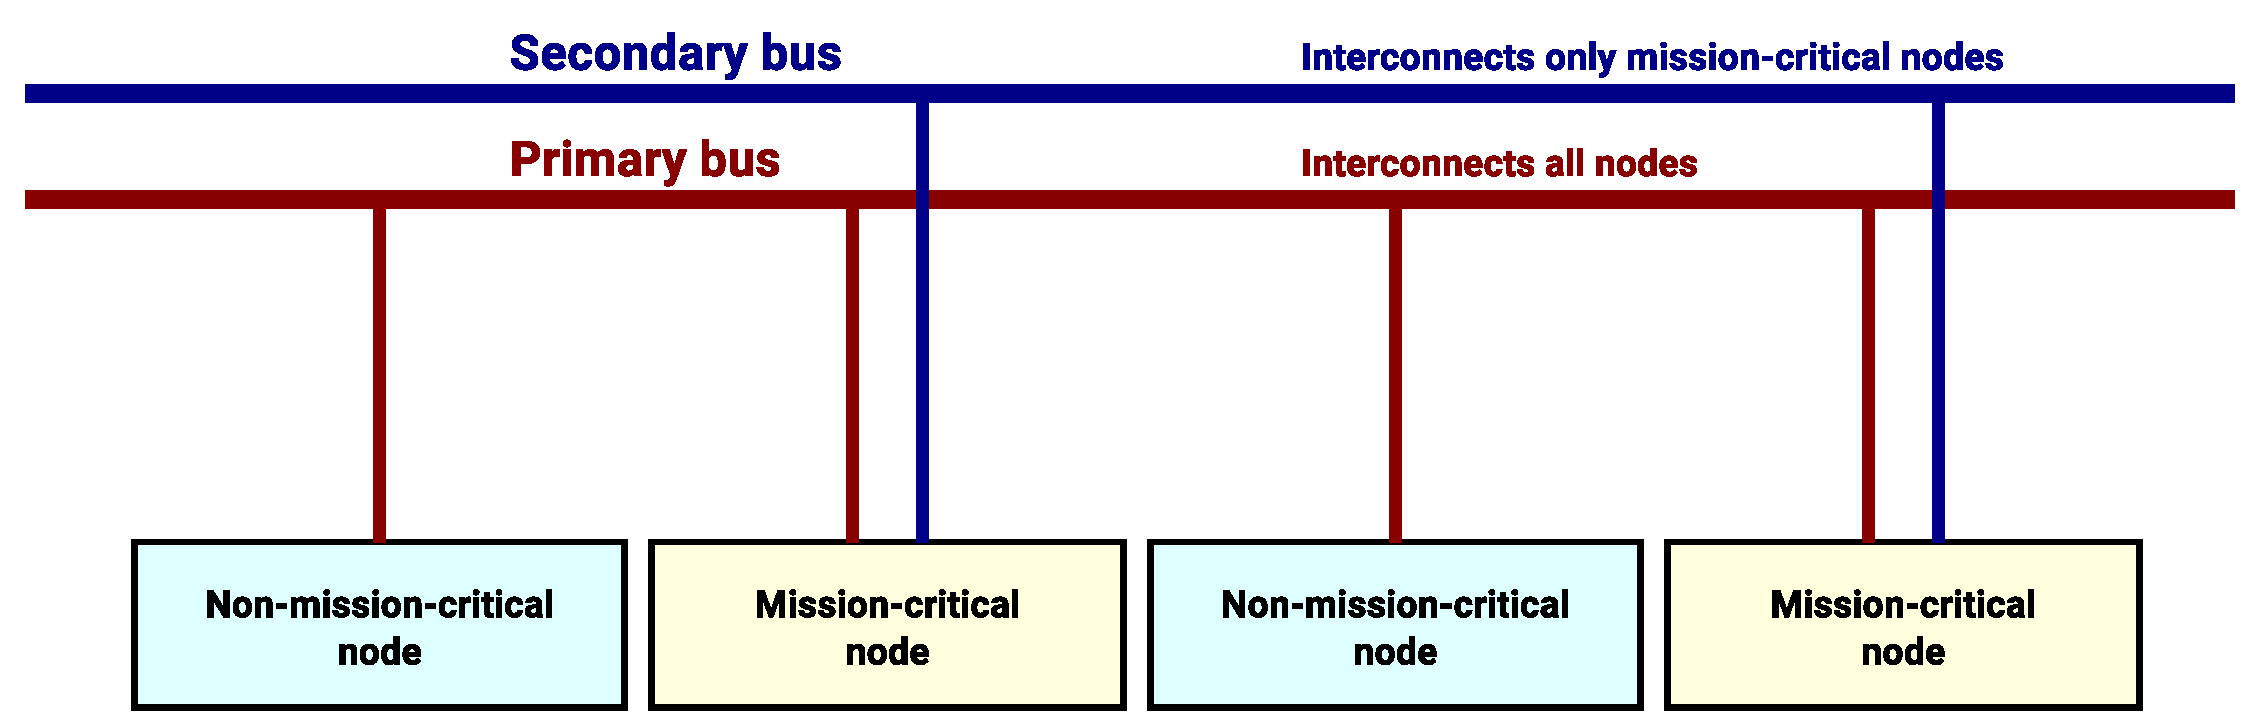
\includegraphics[width=\textwidth]{physical_layer/non_uniform_bus_redundancy}
	\caption{Non-uniform transport redundancy.\label{fig:phy_non_uniform_transport_redundancy}}
\end{figure}

\subsection{Bus power supply}

The standard UAVCAN physical layers support power distribution between nodes.
Integration of the power distribution functionality with the communication interface
removes the need for a dedicated power distribution network,
which greatly simplifies the system design and reduces the complexity and weight of the wiring harnesses.
Additionally, redundant power supply topologies can be easily implemented on top of redundant communication interfaces.

\subsubsection{Power sinking nodes}

This section applies to nodes that draw power from the network.

Each power input should be protected with an over-current protection circuit (for example, an electronic fuse),
so that a short-circuit or a similar failure of the node does not propagate to the entire bus.

If the node incorporates redundant bus interfaces,
it should prevent direct current flow between power inputs from different interface connectors,
so if one bus suffers a power failure (e.g. a short circuit) it is not propagated to the other buses.

\begin{figure}[H]
    \centering
	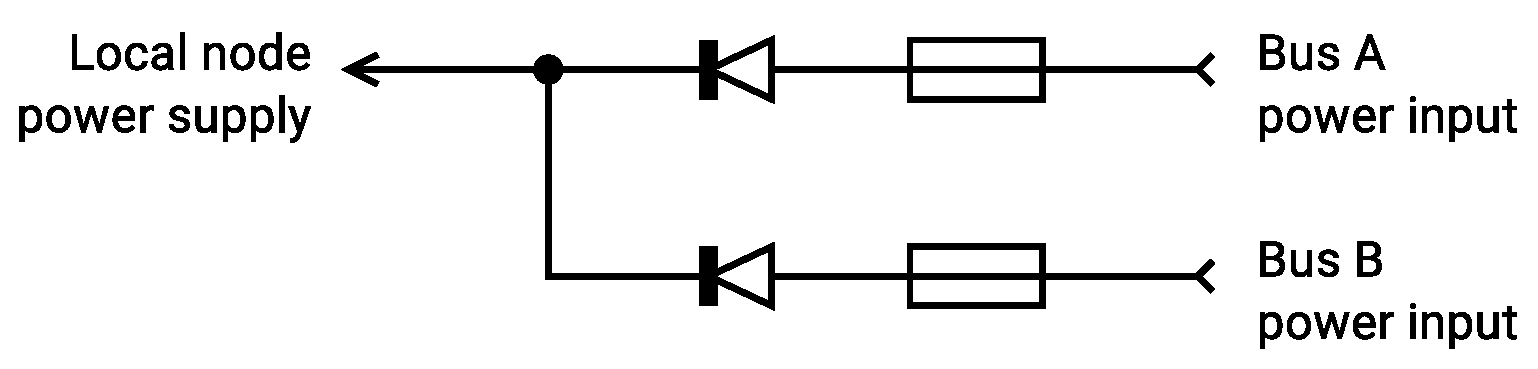
\includegraphics[width=0.6\textwidth]{physical_layer/redundant_bus_power_sink}
	\caption{Simplified conceptual power sinking node design schematic.\label{fig:phy_redundant_bus_power_sink}}
\end{figure}

\subsubsection{Power sourcing nodes}

This section applies to nodes that deliver power to the network.

Similar to the case of bus-powered nodes,
UAVCAN power sources should take into account that one of the redundant interfaces may suffer a
short-circuit or a failure of a similar mode.
Should that happen, the power source should shut down the power supply of the failing bus and continue supplying
the remaining bus interfaces.

\begin{figure}[H]
    \centering
	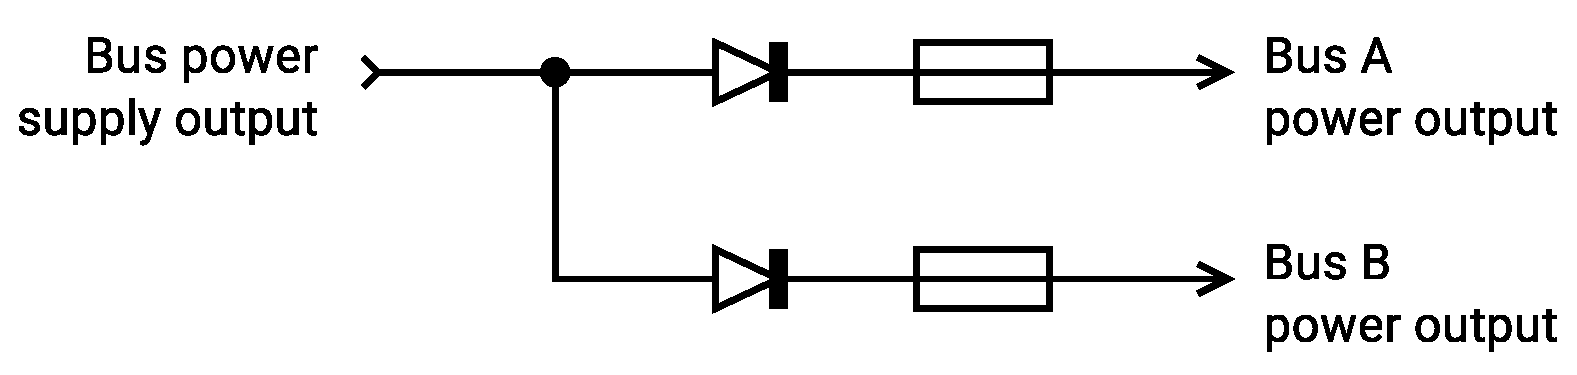
\includegraphics[width=0.6\textwidth]{physical_layer/redundant_bus_power_source}
	\caption{Simplified conceptual power sourcing node design schematic.\label{fig:phy_redundant_bus_power_source}}
\end{figure}
